\documentclass[10pt,twocolumn]{article}
% Shared two-column preamble for the three research papers.
% Use with: \documentclass[10pt,twocolumn]{article}
% Then in main.tex: % Shared two-column preamble for the three research papers.
% Use with: \documentclass[10pt,twocolumn]{article}
% Then in main.tex: % Shared two-column preamble for the three research papers.
% Use with: \documentclass[10pt,twocolumn]{article}
% Then in main.tex: \input{../../shared/latex/twocolumn_preamble.tex}

\usepackage[margin=0.75in]{geometry}
\usepackage[utf8]{inputenc}
\usepackage[T1]{fontenc}
\usepackage{lmodern}
\usepackage{microtype}
\usepackage{amsmath,amssymb,amsthm}
\usepackage{graphicx}
\usepackage{booktabs}
\usepackage{caption}
\usepackage{subcaption}
\usepackage{hyperref}
\usepackage{url}
\usepackage{xcolor}
\usepackage{algorithm}
\usepackage{algorithmic}
\usepackage{multirow}
\usepackage{titlesec}
\usepackage{authblk}

\hypersetup{colorlinks=true,linkcolor=blue!50!black,citecolor=blue!50!black,urlcolor=blue!50!black}

\titleformat{\section}{\normalfont\large\bfseries}{\thesection}{0.6em}{}
\titleformat{\subsection}{\normalfont\bfseries}{\thesubsection}{0.5em}{}

\captionsetup{font=small,labelfont=bf,skip=4pt}
\setlength{\columnsep}{0.25in}
\setlength{\parskip}{2pt}

\newtheorem{theorem}{Theorem}
\newtheorem{proposition}[theorem]{Proposition}
\newtheorem{definition}[theorem]{Definition}


\usepackage[margin=0.75in]{geometry}
\usepackage[utf8]{inputenc}
\usepackage[T1]{fontenc}
\usepackage{lmodern}
\usepackage{microtype}
\usepackage{amsmath,amssymb,amsthm}
\usepackage{graphicx}
\usepackage{booktabs}
\usepackage{caption}
\usepackage{subcaption}
\usepackage{hyperref}
\usepackage{url}
\usepackage{xcolor}
\usepackage{algorithm}
\usepackage{algorithmic}
\usepackage{multirow}
\usepackage{titlesec}
\usepackage{authblk}

\hypersetup{colorlinks=true,linkcolor=blue!50!black,citecolor=blue!50!black,urlcolor=blue!50!black}

\titleformat{\section}{\normalfont\large\bfseries}{\thesection}{0.6em}{}
\titleformat{\subsection}{\normalfont\bfseries}{\thesubsection}{0.5em}{}

\captionsetup{font=small,labelfont=bf,skip=4pt}
\setlength{\columnsep}{0.25in}
\setlength{\parskip}{2pt}

\newtheorem{theorem}{Theorem}
\newtheorem{proposition}[theorem]{Proposition}
\newtheorem{definition}[theorem]{Definition}


\usepackage[margin=0.75in]{geometry}
\usepackage[utf8]{inputenc}
\usepackage[T1]{fontenc}
\usepackage{lmodern}
\usepackage{microtype}
\usepackage{amsmath,amssymb,amsthm}
\usepackage{graphicx}
\usepackage{booktabs}
\usepackage{caption}
\usepackage{subcaption}
\usepackage{hyperref}
\usepackage{url}
\usepackage{xcolor}
\usepackage{algorithm}
\usepackage{algorithmic}
\usepackage{multirow}
\usepackage{titlesec}
\usepackage{authblk}

\hypersetup{colorlinks=true,linkcolor=blue!50!black,citecolor=blue!50!black,urlcolor=blue!50!black}

\titleformat{\section}{\normalfont\large\bfseries}{\thesection}{0.6em}{}
\titleformat{\subsection}{\normalfont\bfseries}{\thesubsection}{0.5em}{}

\captionsetup{font=small,labelfont=bf,skip=4pt}
\setlength{\columnsep}{0.25in}
\setlength{\parskip}{2pt}

\newtheorem{theorem}{Theorem}
\newtheorem{proposition}[theorem]{Proposition}
\newtheorem{definition}[theorem]{Definition}

\newcommand{\DetNPerClass}{300}
\newcommand{\DetNTrain}{840}
\newcommand{\DetNTest}{360}
\newcommand{\DetGbFBest}{0.969}
\newcommand{\DetGbFBestFs}{200}
\newcommand{\DetGbFHundred}{0.947}
\newcommand{\DetGbFOneK}{0.936}
\newcommand{\DetThrFBest}{0.666}
\newcommand{\DetThrFMin}{0.547}
\newcommand{\DetThrFMax}{0.666}
\newcommand{\DetConsFHundred}{0.879}
\newcommand{\DetConsFBest}{0.961}
\newcommand{\DetConsClipPct}{66}
\newcommand{\DetPamGbSport}{0.908}
\newcommand{\DetPamGbCons}{0.874}
\newcommand{\DetPamThrSport}{0.630}
\newcommand{\DetPamSegments}{10}
\newcommand{\TimBallOneK}{0.52}
\newcommand{\TimBallFiveH}{2.15}
\newcommand{\TimBallHundred}{5.8}
\newcommand{\TimPlayerOneK}{14.8}
\newcommand{\TimPlayerMadOneK}{2.1}
\newcommand{\TimPlayerHundred}{22.4}
\newcommand{\OrdSigmaOneK}{1.3}
\newcommand{\OrdSigmaHundred}{5.9}
\newcommand{\OrdSigmaBall}{1.2}
\newcommand{\OrdGapNinetyOneK}{20}
\newcommand{\OrdGapNinetyHundred}{20}
\newcommand{\OrdPTenOneK}{0.88}
\newcommand{\OrdPTenHundred}{0.64}
\newcommand{\OrdPTwoOneK}{0.61}
\newcommand{\OvlAccThree}{0.58}
\newcommand{\OvlAccSix}{0.73}
\newcommand{\OvlAccTen}{0.88}
\newcommand{\OvlAccFifteen}{0.96}
\newcommand{\OvlAccTwenty}{1.00}
\newcommand{\OvlAccZero}{0.63}
\newcommand{\OvlTwoMin}{0.96}
\newcommand{\OvlGbBothMin}{0.84}
\newcommand{\OvlGbBothMax}{0.96}
\newcommand{\OvlGapRmseWide}{6}
\newcommand{\OvlGapRmseNarrow}{15}
\newcommand{\OvlNPerGap}{120}
\newcommand{\OvlFs}{1000}
\newcommand{\DecPriorAcc}{0.667}
\newcommand{\DecPriorBrier}{0.218}
\newcommand{\DecPriorEce}{0.020}
\newcommand{\DecPriorAccSingle}{0.656}
\newcommand{\DecPriorAccBoth}{0.677}
\newcommand{\DecBootAcc}{0.809}
\newcommand{\DecBootBrier}{0.123}
\newcommand{\DecBootEce}{0.029}
\newcommand{\DecBootAccSingle}{1.000}
\newcommand{\DecBootAccBoth}{0.616}
\newcommand{\DecBootPriorAcc}{0.825}
\newcommand{\DecBootPriorBrier}{0.112}
\newcommand{\DecBootPriorEce}{0.035}
\newcommand{\DecBootPriorAccSingle}{0.995}
\newcommand{\DecBootPriorAccBoth}{0.653}
\newcommand{\DecBootBallAcc}{0.951}
\newcommand{\DecBootBallBrier}{0.049}
\newcommand{\DecBootBallEce}{0.046}
\newcommand{\DecBootBallAccSingle}{0.971}
\newcommand{\DecBootBallAccBoth}{0.930}
\newcommand{\DecAllAcc}{0.927}
\newcommand{\DecAllBrier}{0.055}
\newcommand{\DecAllEce}{0.054}
\newcommand{\DecAllAccSingle}{0.915}
\newcommand{\DecAllAccBoth}{0.938}
\newcommand{\DecStackAcc}{0.944}
\newcommand{\DecStackBrier}{0.038}
\newcommand{\DecStackEce}{0.031}
\newcommand{\DecStackAccSingle}{0.942}
\newcommand{\DecStackAccBoth}{0.946}
\newcommand{\DecNCases}{1500}
\newcommand{\DecNEval}{750}
\newcommand{\DecBaseRate}{0.59}
\newcommand{\DecBest}{all stacked}
\newcommand{\DecReviewRate}{5}
\newcommand{\DecErrDecided}{3.4}
\newcommand{\DecErrNoReview}{5.6}
\newcommand{\DecThrFour}{0.20}
\newcommand{\DecFalseFoulFour}{0.7}
\newcommand{\DecFalseFoulOne}{4.1}
\newcommand{\DecMissedFour}{6.7}
\newcommand{\DecMissedOne}{1.5}
\newcommand{\DecCoefBoot}{1.68}
\newcommand{\DecCoefBall}{0.41}
\newcommand{\DecCoefSep}{1.29}
\newcommand{\DecCoefPrior}{0.83}
\newcommand{\DecLateAccAll}{0.96}
\newcommand{\DecLateAccPrior}{0.78}
\newcommand{\LocFreeSport}{3.3}
\newcommand{\LocZuptSport}{0.77}
\newcommand{\LocFreeCons}{7.6}
\newcommand{\LocZuptCons}{1.98}
\newcommand{\LocUwbOneSport}{0.27}
\newcommand{\LocUwbFiveSport}{0.15}
\newcommand{\LocUwbTwentySport}{0.09}
\newcommand{\LocUwbTwentyCons}{0.12}
\newcommand{\LocUwbTenSport}{0.12}
\newcommand{\LocWrongHalfTen}{0.00}
\newcommand{\LocWrongQuarterTen}{1.7}
\newcommand{\LocWrongTenTen}{20}
\newcommand{\LocWrongHalfZupt}{26}
\newcommand{\LocUwbSigma}{0.10}
\newcommand{\LocNRuns}{20}
\newcommand{\LocDuration}{6}
\newcommand{\LocSpeed}{6}


\title{Who Touched First? Detecting, Ordering and Placing Boot--Ball and
Boot--Player Contacts from a Shoe-Mounted Inertial Sensor}
\author[1]{Luis Benvenuto}
\affil[1]{Independent Research}
\date{September 14, 2026}

\begin{document}
\twocolumn[
\maketitle
\begin{@twocolumnfalse}
\begin{abstract}
\noindent The connected match ball detects the instant it is struck from an
inertial sensor suspended at its centre. A foul is decided by the other half of
that event: what the boot hit, and in which order. We ask whether a
boot-mounted inertial measurement unit (IMU) can supply that half. Because no
public recording of instrumented fouls exists, we build a physics-based
simulator of the boot's signal --- a running gait with foot strikes, a short
stiff ball impact with post-impact ringing, a longer softer oblique player
contact with a push tail, and their near-simultaneous superposition --- passed
through a sensor model (bandwidth, noise, bias, full-scale clipping, sampling
rate), with real ankle-IMU recordings of walking, running and playing football
(PAMAP2) as an alternative background. Four results follow. (i) A
gradient-boosting classifier on interpretable pulse features separates
\{none, ball, player, both\} at macro-F1 \DetGbFBest\ on synthetic and
\DetPamGbSport\ on real background, against \DetThrFMin--\DetThrFMax\ for the
ball-style threshold rule; a $\pm16$\,g phone-grade part clips
\DetConsClipPct\% of ball impacts yet still reaches \DetConsFBest. (ii) The
ball-contact onset is timed to \TimBallOneK\,ms at 1\,kHz (\TimBallHundred\,ms
at 100\,Hz), and combining it with the ball's own sensor orders a ball contact
and a player contact correctly at $\geq 90$\% once they are
\OrdGapNinetyOneK\,ms apart. (iii) In the anomalous case where the boot hits
ball and opponent inside one pulse width, a two-template non-negative
least-squares separator recovers the order in \OvlAccTen\ of cases at 10\,ms
and \OvlAccTwenty\ at 20\,ms, but is at chance below 3\,ms --- a physical
limit, not an algorithmic one. (iv) Fusing boot posterior, ball-sensor timing,
separator order and a knowledge base of situational base rates in a
calibrated stacked model yields a \emph{probability} that the ball was played
first with accuracy \DecStackAcc\ and Brier score \DecStackBrier\ (prior
alone: \DecPriorAcc\ / \DecPriorBrier), from which a cost-weighted rule with a
review band decides fouls at \DecErrDecided\% error while referring
\DecReviewRate\% of cases. Finally, foot-mounted inertial navigation with
zero-velocity updates and sparse ultra-wideband fixes places the contact
within \LocUwbTenSport\,m at 10\,Hz, enough to make a penalty-area call
wrong with probability \LocWrongQuarterTen\% at 25\,cm from the line. The
pipeline is configuration-driven and reproduces in minutes on a laptop.
\end{abstract}
\vspace{1em}
\end{@twocolumnfalse}
]

\section{Introduction}
\label{sec:intro}

Modern football already instruments one of the two bodies in every contact.
The match ball used at the 2022 World Cup carries an inertial sensor suspended
at its centre, sampled at 500\,Hz, whose sudden change of acceleration marks
the instant the ball is touched; that timestamp, fused with limb tracking from
cameras, is what made semi-automated offside possible and what settled whether
a striker's head had grazed a goal-bound cross \cite{fifa2022connected}. The
ball, in other words, knows \emph{when} it was hit. It does not know
\emph{what} hit it, nor whether the boot that hit it had struck an opponent a
few milliseconds earlier --- which is precisely the question a referee must
answer to call a foul.

This paper asks whether the other body in the contact can be instrumented in
the same spirit. A small IMU in the boot (in the heel counter or under the
insole) sees every impact the foot delivers. Three signatures matter: the
\emph{ball}, a short, hard, forward-axis deceleration (foot--ball contact lasts
about ten milliseconds \cite{nunome2006impact}) followed by a high-frequency
ringing from the stiff boot--ball interface; the \emph{player}, a longer,
softer, oblique pulse as soft tissue compresses, followed by a low-frequency
push as the bodies keep moving into each other; and the \emph{ground}, a
periodic, mostly vertical foot strike that is the boot's normal background.
The interesting --- and contested --- case is the fourth: the boot hits ball and
opponent almost at once, and the call turns on which came first.

We treat this as a measurement problem with a decision-theoretic ending, and
we answer it by simulation. There is no public dataset of instrumented fouls,
so we build a physics-based generator for the boot's signal and pass it through
an explicit sensor model, using real ankle-IMU recordings of walking, running
and playing football \cite{reiss2012introducing} as an alternative background
to check that the synthetic gait is not doing the work. The study then runs in
four stages:

\begin{enumerate}
\item \textbf{Detection.} Can the boot tell ball from player from ground, and
  at what sampling rate and sensor grade? We compare the threshold logic of a
  connected ball (``a sudden change of the acceleration vector'') with a
  gradient-boosting classifier on interpretable pulse features.
\item \textbf{Timing and ordering.} How precisely is a contact onset timed,
  and --- combining the boot with the ball's own sensor --- how far apart must a
  ball contact and a player contact be for their order to be recovered?
\item \textbf{The anomalous overlap.} When both pulses fall inside one pulse
  width, a two-template non-negative least-squares fit separates them; we map
  where it works and where the physics says nothing can.
\item \textbf{The probabilistic call.} A knowledge base of situational base
  rates (how often a sliding tackle plays the ball first) is fused with the
  boot posterior, the ball-sensor timing and the separator's order into a
  calibrated probability that the ball was played first, and a cost-weighted
  rule with a video-review band decides.
\end{enumerate}
A fifth section places the contact in space: foot-mounted inertial navigation
with zero-velocity updates \cite{foxlin2005pedestrian} and sparse
ultra-wideband anchor fixes, evaluated as the probability of putting a contact
on the wrong side of the penalty-area line.

Our contribution is a quantified map of what a boot sensor can and cannot
settle, not a product. The numbers are specific to a simulator whose
assumptions we state and whose knobs we expose; every figure and every number
in the text regenerates from one command.

\section{Related work}
\label{sec:related}

\paragraph{Instrumented balls and officiating.} The connected ball
\cite{fifa2022connected} embeds a 500\,Hz IMU whose impact detection, fused
with optical limb tracking, feeds semi-automated offside and has been used to
adjudicate touches. Our ball-sensor model (a detected impact time with a
clock-sync error and sample quantisation) is an abstraction of that device; the
boot sensor is the missing complement.

\paragraph{Kicking biomechanics.} Foot--ball contact in the instep kick lasts
roughly 8--12\,ms with foot speeds of 15--25\,m/s \cite{nunome2006impact,
lees1998biomechanics}; the foot decelerates by tens of $g$ over that interval,
which is why impact-rated accelerometers ($\pm 200$\,g) are used in kicking
studies and why a $\pm16$\,g consumer part clips. These figures set the ball
template in our simulator.

\paragraph{Inertial sensing and change detection.} Sensor error models (white
noise, bias, bandwidth) follow the standard inertial-navigation treatment
\cite{woodman2007introduction}. Onset estimation uses a threshold crossing
with sub-sample interpolation and a matched filter on the pulse's rising edge
\cite{turin1960introduction}; two-pulse separation is non-negative least
squares \cite{lawson1974solving} over a lag grid with a BIC-like penalty for
the second pulse.

\paragraph{Activity recognition from wearable IMUs.} PAMAP2
\cite{reiss2012introducing} provides ankle-mounted IMU recordings including
running and playing football; we use it strictly as background under which
synthetic contacts are injected. Gradient boosting \cite{friedman2001greedy}
on hand-crafted features is the classical strong baseline for such windows.

\paragraph{Calibrated probabilities and decisions.} Isotonic calibration
\cite{zadrozny2002transforming}, the Brier score \cite{brier1950verification}
and expected calibration error are the standard tools for asking whether a
probability is honest; stacked generalisation \cite{wolpert1992stacked} is the
standard fix when naively fused sources are correlated. The decision rule is
Bayes-optimal thresholding under asymmetric costs with an abstention band,
which is how a video-review protocol is naturally formalised.

\paragraph{Foot-mounted navigation.} Zero-velocity updates during stance make
shoe-mounted inertial navigation drift linearly rather than cubically
\cite{foxlin2005pedestrian, skog2010zero}; ultra-wideband anchors bound the
remaining drift \cite{alarifi2016ultra}. We combine both in a small Kalman
filter \cite{kalman1960new} and score the error where it matters: at the
contact, against a line on the pitch.

\section{Method}
\label{sec:method}

\subsection{Simulating the boot's signal}
Signals are generated at 4\,kHz in the boot's frame ($x$ forward, $y$
lateral, $z$ sole normal) and then passed through the sensor model. The
\emph{gait} is a running stride (2.4--3.2 strides/s): smooth swing-phase
acceleration, a vertical half-sine foot strike (6--14\,g, 25--40\,ms) with a
braking component, foot pitch that rotates gravity in the sensor frame, and
the corresponding angular rate. Three \emph{events} are injected at a random
instant:
\begin{itemize}
\item \textbf{ball}: a half-sine deceleration along $-x$ with peak
  50--130\,g and duration 7--12\,ms \cite{nunome2006impact}, followed by a
  damped 150--260\,Hz ringing at 18\% of the peak;
\item \textbf{player}: an oblique half-sine of 8--45\,g lasting 18--55\,ms,
  followed by a 0.5--3\,g push tail over 60--160\,ms, with a lateral twist on
  the gyroscope;
\item \textbf{both}: a ball pulse and a player pulse separated by a signed gap
  (negative: the player was hit first).
\end{itemize}
Figure~\ref{fig:sig} shows one sampled window of each class.

\begin{figure}[t]
\centering
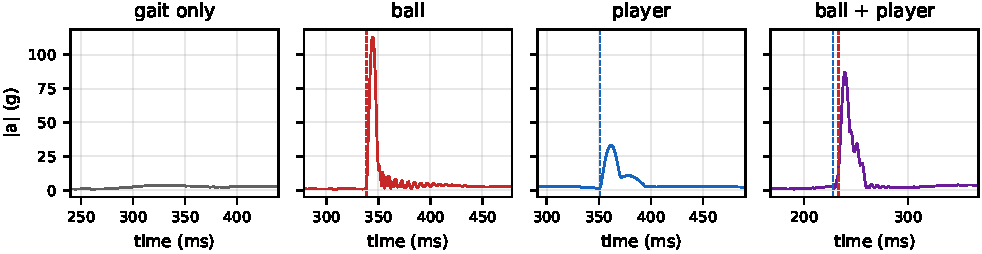
\includegraphics[width=\columnwidth]{figures/signatures.pdf}
\caption{Acceleration magnitude of one window per class at 1\,kHz (impact-rated
sensor). Dashed lines mark the true ball (red) and player (blue) onsets. The
ball is short, hard and rings; the player is longer, softer and pushes; in the
overlap both sit inside one pulse width.}
\label{fig:sig}
\end{figure}

\subsection{Sensor model and real background}
The sensor chain is a first-order low-pass at 45\% of Nyquist, a constant
bias, white noise scaled with $\sqrt{f_s}$, clipping at full scale, and
decimation to the sampling rate $f_s$. Two parts are modelled: an
impact-rated \emph{sport} accelerometer ($\pm200$\,g) and a phone-grade
\emph{consumer} one ($\pm16$\,g). The \emph{ball sensor} reports an impact time
only when the ball is struck, quantised to its 500\,Hz grid with a 1\,ms clock
offset to the boot. As an alternative background we crop real 100\,Hz
ankle-IMU segments of walking, running and playing football from PAMAP2
\cite{reiss2012introducing} (\DetPamSegments\ subject--activity segments) and
inject the same synthetic events; because those recordings contain nothing
above 50\,Hz, the real background is only used at its native rate.

\subsection{Detectors}
\paragraph{Features.} Sixteen pulse descriptors of a window: peak
$|\mathbf a|$ and peak jerk, widths at half and tenth maximum, high-frequency
energy ratio and spectral centroid around the peak, zero crossings of the
post-peak tail (ringing), direction cosines of the peak, gyroscope peaks,
kurtosis, mean of the 40--120\,ms tail (push), background RMS, and the number
of secondary peaks.
\paragraph{Threshold rule.} The connected-ball logic: contact if the peak
exceeds $\tau$; ball if the half-maximum width is below $w$, else player; both
if a second comparable peak exists. $(\tau,w)$ are grid-searched on the
training split, so this baseline is as strong as a threshold rule can be.
\paragraph{Boosting.} Histogram gradient boosting \cite{friedman2001greedy} on
the same features, returning class probabilities.
\paragraph{Onset.} Two estimators anchored on the peak of the \emph{horizontal}
excess (foot strikes are vertical, contacts are not): the first sample above
$\max(6\sigma, 0.08\,\text{peak})$ walking back from the peak, refined by
linear interpolation; and a matched filter on the rising edge of a clean
template with a parabolic sub-sample fit \cite{turin1960introduction}.
\paragraph{Separator.} For the overlap, $|\mathbf a| - \text{baseline}$ is fit
as $A\,T_{\text{ball}}(t-t_1) + B\,T_{\text{player}}(t-t_2)$, $A,B\ge 0$, over a
lag grid, with the closed-form two-column non-negative least-squares solution
\cite{lawson1974solving} vectorised across all $(t_1,t_2)$; a BIC-like penalty
decides whether a second pulse is warranted. The output is the model
(ball/player/both), both onsets, the signed gap and the order.

\subsection{From evidence to a probability}
For a challenge with situation $s$ (standing tackle, sliding tackle, 50/50,
late challenge) the \emph{knowledge base} supplies a base rate
$\pi_s = P(\text{ball first}\mid s)$; the rates used here are illustrative and
are a configuration table. Three sensor sources produce a score in $[0,1]$:
the boosting posterior $P(\text{ball}) + \tfrac12 P(\text{both})$; the
\emph{timing} score $1-\Phi\!\big((\hat t_{\text{ball}} - \hat
t_{\text{boot,first}})/(\sigma\sqrt2)\big)$ from the ball sensor's time against
the boot's first onset, and $0$ if the ball reports nothing; and the
separator's order with confidence $\Phi(|\hat\Delta|/(\sigma\sqrt2))$. Each
score is isotonically calibrated on a held-out half
\cite{zadrozny2002transforming}. Two fusions are compared: the naive-Bayes
log-odds sum $\operatorname{logit}\pi_s + \sum_k
[\operatorname{logit} p_k - \operatorname{logit}\bar p]$, and a stacked
logistic regression on the calibrated log-odds \cite{wolpert1992stacked}. The
\emph{decision} calls ``no foul'' when $P(\text{ball first}) > c_{\text{miss}} /
(c_{\text{false}} + c_{\text{miss}})$, and refers the case to review when the
posterior lies within a band of that threshold.

\subsection{Placing the contact}
A 6-state Kalman filter on position and velocity integrates the world-frame
acceleration obtained from gyro-integrated orientation, with zero-velocity
updates whenever the foot looks planted ($|\boldsymbol\omega| < 40^\circ$/s
and $|\mathbf f| \approx g$) \cite{foxlin2005pedestrian, skog2010zero} and
ultra-wideband position fixes ($\sigma = \LocUwbSigma$\,m) at a configurable
rate. The trajectory is a \LocSpeed\,m/s run with a lateral cut over
\LocDuration\,s; error is scored over the second half of the run. The
probability of misplacing a contact at distance $d$ from a line is
$\Phi(-d/\sigma_{\text{pos}})$.

\section{Detection and timing}
\label{sec:detect}

\begin{figure*}[t]
\centering
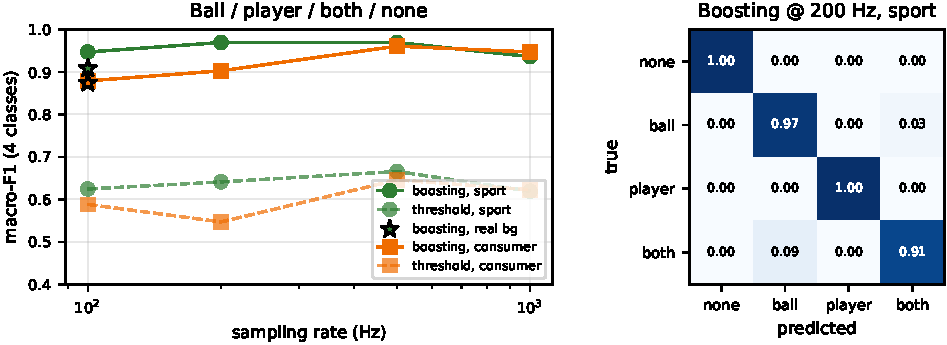
\includegraphics[width=\textwidth]{figures/detect.pdf}
\caption{Left: four-class macro-F1 versus sampling rate for the boosting
classifier (solid) and the tuned threshold rule (dashed), for an impact-rated
(green) and a phone-grade $\pm16$\,g (orange) sensor on synthetic background;
stars are boosting on real PAMAP2 ankle-IMU background at its native 100\,Hz.
Right: the boosting confusion matrix at its best rate. The only systematic
confusion is \emph{both} $\to$ \emph{ball}: when the player pulse is faint the
overlap looks like a clean kick.}
\label{fig:detect}
\end{figure*}

\paragraph{Classification.} Figure~\ref{fig:detect} answers the first
question. With \DetNPerClass\ windows per class (\DetNTrain\ train /
\DetNTest\ test), boosting reaches macro-F1 \DetGbFBest\ at
\DetGbFBestFs\,Hz and stays between \DetGbFOneK\ and \DetGbFBest\ across
100--1000\,Hz; the threshold rule, even with its two thresholds tuned, sits at
\DetThrFMin--\DetThrFMax. The gap is not about detecting \emph{that} something
was hit --- both do that --- but about \emph{what}: a single peak-and-width
rule cannot represent ringing, push tails, direction and secondary peaks at
once. The phone-grade sensor clips \DetConsClipPct\% of the ball impacts, and
at 100\,Hz this costs it (F1 \DetConsFHundred), but by 500\,Hz the shape of
the clipped plateau, the ringing and the direction carry enough information to
recover to \DetConsFBest: full scale matters less than sampling rate. On real
ankle-IMU background at 100\,Hz boosting reaches \DetPamGbSport\ (sport) and
\DetPamGbCons\ (consumer), close to the synthetic values at the same rate,
which says the synthetic gait is not making the task artificially easy; the
threshold rule on real background is \DetPamThrSport.

\begin{figure*}[t]
\centering
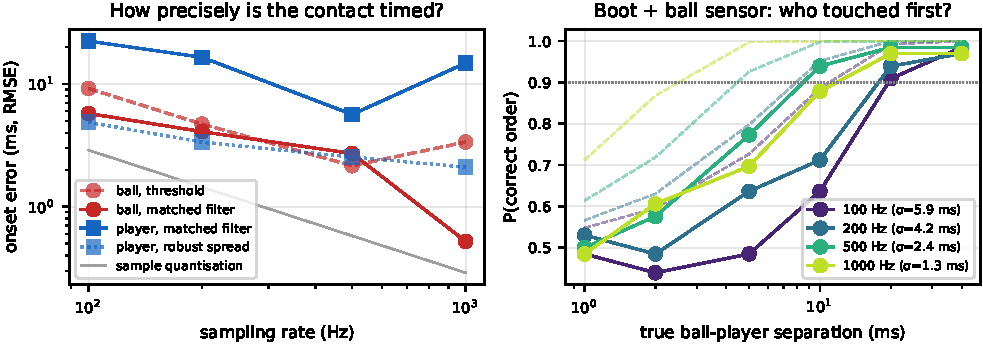
\includegraphics[width=\textwidth]{figures/timing.pdf}
\caption{Left: onset error versus sampling rate (noise at nominal). The ball's
onset follows sample quantisation down to sub-millisecond; the player's RMSE is
dominated by a few gross errors (a faint contact mistaken for a foot strike),
its robust spread is a few ms. Right: probability of correctly ordering a ball
contact and a player contact from the boot's first onset and the ball sensor's
time, versus their true separation, at each rate; dashed lines are the closed
form $\Phi(\Delta/(\sigma\sqrt2))$ with the measured $\sigma$.}
\label{fig:timing}
\end{figure*}

\paragraph{Timing.} The ball onset is timed to \TimBallOneK\,ms RMSE at
1\,kHz, \TimBallFiveH\,ms at 500\,Hz and \TimBallHundred\,ms at 100\,Hz; the
matched filter's parabolic refinement beats the sample grid at high rates,
the threshold crossing is better at low ones (Figure~\ref{fig:timing}, left).
The player onset is intrinsically softer: its robust spread is
\TimPlayerMadOneK\,ms at 1\,kHz but its RMSE (\TimPlayerOneK\,ms) is
dominated by a few percent of gross errors where a weak contact is out-shouted
by a foot strike. Anchoring the estimator on the horizontal component of the
acceleration (foot strikes are vertical) is what brings those gross errors from
tens of percent to a few.

\paragraph{Who touched first, from two clocks.} Given the boot's first onset
and the ball sensor's time, ``ball first'' is declared when the ball fired
within $2\sigma$ of the boot onset, where $\sigma$ combines the boot timing
error with the ball's clock offset and sample quantisation (\OrdSigmaBall\,ms).
The right panel of Figure~\ref{fig:timing} plots the empirical probability of a
correct order against the true separation. At 1\,kHz the combined
$\sigma$ is \OrdSigmaOneK\,ms, the order is right in \OrdPTenOneK\ of cases at
10\,ms and passes 90\% at \OrdGapNinetyOneK\,ms; at 100\,Hz
($\sigma=\OrdSigmaHundred$\,ms) it is \OrdPTenHundred\ at 10\,ms. Below
2--3\,ms every rate is at chance (\OrdPTwoOneK\ at 2\,ms, 1\,kHz). The closed
form with independent Gaussian errors is optimistic at small gaps --- the two
onsets are not independent when the pulses overlap, which is the subject of
the next section --- and matches well once the pulses are distinct.

\section{The overlap, and the probabilistic call}
\label{sec:decision}

\begin{figure*}[t]
\centering
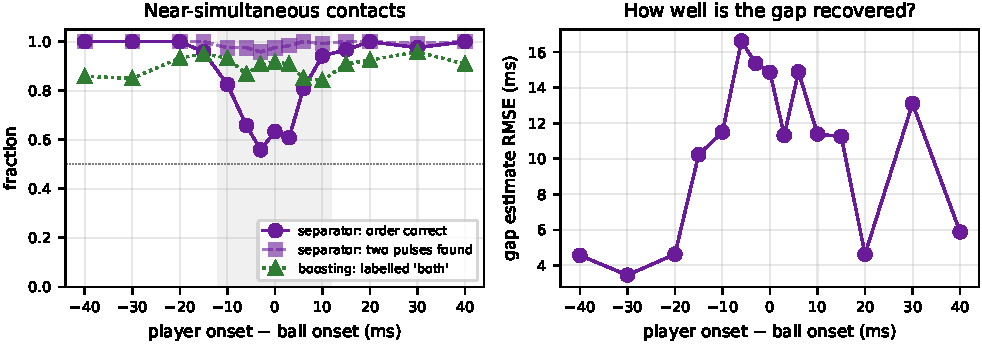
\includegraphics[width=\textwidth]{figures/overlap.pdf}
\caption{The anomalous case: ball and player struck within one window, versus
the signed gap (player onset minus ball onset; negative = player first). Left:
the separator finds two pulses almost always and orders them correctly outside
the shaded band (one ball-pulse duration), while the boosting classifier
labels the window \emph{both} at a roughly constant rate regardless of gap.
Right: RMSE of the recovered gap.}
\label{fig:overlap}
\end{figure*}

\paragraph{The anomalous overlap.} Figure~\ref{fig:overlap} maps the case the
project was started for: the boot hits the opponent and the ball inside one
pulse width. With \OvlNPerGap\ windows per gap at \OvlFs\,Hz, the two-template
separator declares two pulses in at least \OvlTwoMin\ of windows at every gap,
and orders them correctly in \OvlAccTwenty\ of cases at $\pm20$\,ms,
\OvlAccFifteen\ at $\pm15$\,ms, \OvlAccTen\ at $\pm10$\,ms, \OvlAccSix\ at
$\pm6$\,ms and \OvlAccThree\ at $\pm3$\,ms (\OvlAccZero\ at zero, which is
chance by construction). The gap itself is recovered to \OvlGapRmseWide\,ms
RMSE when the pulses are 20\,ms or more apart and only to
\OvlGapRmseNarrow\,ms inside the overlap. The boosting classifier, by contrast,
labels \OvlGbBothMin--\OvlGbBothMax\ of these windows \emph{both} at every gap:
it knows two things were hit but has no notion of order. The shape of the
left panel is the physical content of this paper: the ball pulse lasts
7--12\,ms, so two contacts closer than that share their rising edges and no
estimator can tell which began first from the boot alone. Above about one
pulse duration the order is recoverable and above two it is essentially
certain.

\begin{figure*}[t]
\centering
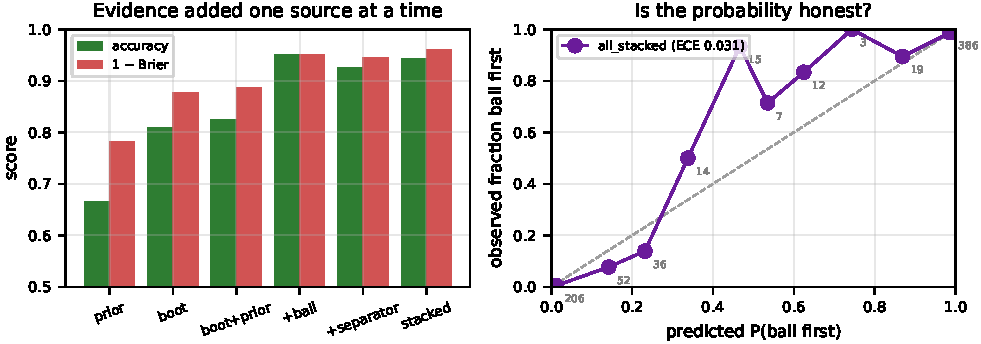
\includegraphics[width=\textwidth]{figures/decision.pdf}
\caption{Left: accuracy and $1-$Brier of $P(\text{ball first})$ as evidence is
added --- knowledge-base prior, boot classifier, ball-sensor timing, separator
order --- with naive-Bayes fusion, and the stacked logistic fusion of all
sources. Right: reliability diagram of the best model (bin counts in grey).}
\label{fig:decision}
\end{figure*}

\paragraph{From evidence to a probability.} Figure~\ref{fig:decision} reports
the decision layer on \DecNEval\ held-out challenges (half clean single
contacts, half overlaps with gaps of 2--40\,ms; base rate of ball-first
\DecBaseRate). The knowledge-base prior alone is right \DecPriorAcc\ of the
time with Brier \DecPriorBrier: base rates are informative but not decisive.
The boot classifier alone reaches \DecBootAcc\ --- essentially perfect on
clean contacts (\DecBootAccSingle) and near chance on overlaps
(\DecBootAccBoth), for the reason just given. Adding the ball sensor's timing
is the step that matters: accuracy \DecBootBallAcc, Brier \DecBootBallBrier,
with overlaps now at \DecBootBallAccBoth. Adding the separator's order under
naive-Bayes fusion \emph{hurts} slightly (\DecAllAcc), because the boot
posterior and the separator read the same window and are double-counted; the
stacked logistic fusion resolves this (accuracy \DecStackAcc, Brier
\DecStackBrier, ECE \DecStackEce), learning weights of \DecCoefBoot\ (boot),
\DecCoefBall\ (ball timing), \DecCoefSep\ (separator) and \DecCoefPrior\
(prior) on the calibrated log-odds. The reliability diagram shows the
probabilities are honest across the range; the situation where the prior is
most wrong (a late challenge, prior \DecLateAccPrior\ accuracy) is where the
sensors help most (\DecLateAccAll).

\paragraph{The call.} With equal costs for a false foul and a missed foul the
threshold is $0.5$ and the error rate is \DecErrNoReview\%; adding a review
band of $\pm0.15$ refers \DecReviewRate\% of challenges to video and lowers the
error among those decided on the field to \DecErrDecided\%. If a false foul is
judged four times as costly as a missed one, the threshold moves to
\DecThrFour\ and false fouls fall from \DecFalseFoulOne\% to
\DecFalseFoulFour\% of challenges while missed fouls rise from
\DecMissedOne\% to \DecMissedFour\%. The point of a calibrated probability is
exactly that this trade is a policy setting, not a retraining.

\section{Where was the contact?}
\label{sec:localize}

\begin{figure*}[t]
\centering
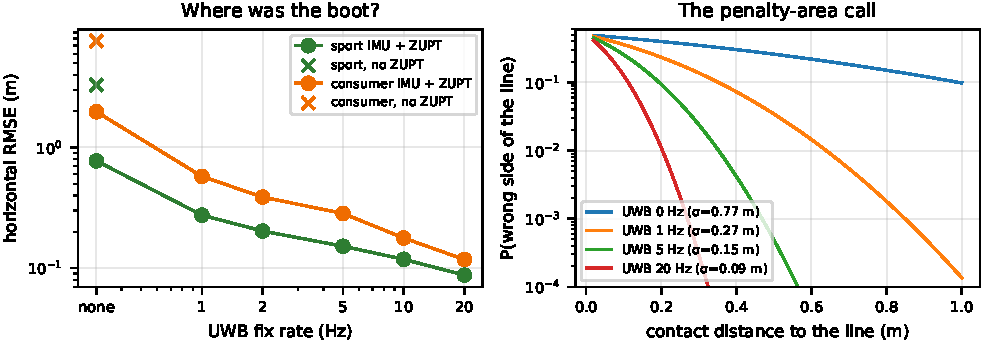
\includegraphics[width=\textwidth]{figures/localize.pdf}
\caption{Left: horizontal position RMSE of the boot over the second half of a
\LocDuration\,s run with a cut, versus ultra-wideband fix rate, for an
impact-rated and a phone-grade IMU with zero-velocity updates (crosses: free
inertial integration). Right: probability of placing a contact on the wrong
side of a line versus its distance to the line, for several fix rates.}
\label{fig:localize}
\end{figure*}

Ordering the contacts says whether a foul happened; placing it says where the
free kick is taken and whether it is a penalty. Figure~\ref{fig:localize}
gives the boot's position error from its own IMU with zero-velocity updates
(ZUPT) and sparse ultra-wideband (UWB) fixes, over \LocNRuns\ runs. Free
inertial integration drifts to \LocFreeSport\,m (sport IMU) and
\LocFreeCons\,m (consumer) horizontally within a few seconds; ZUPT alone brings
this to \LocZuptSport\,m and \LocZuptCons\,m, because every stance resets
velocity and drift accumulates per stride rather than per second
\cite{foxlin2005pedestrian}. One UWB fix per second is worth more than the
IMU grade: \LocUwbOneSport\,m for the sport part, and at 10\,Hz
\LocUwbTenSport\,m, at 20\,Hz \LocUwbTwentySport\,m (consumer:
\LocUwbTwentyCons\,m) --- close to the \LocUwbSigma\,m of the anchors
themselves, at which point the filter is interpolating between fixes with the
IMU rather than dead-reckoning.

Read as a decision, the right panel is the penalty-area call. With 10\,Hz
fixes a contact 25\,cm outside the line is placed inside with probability
\LocWrongQuarterTen\%, at 10\,cm the probability is \LocWrongTenTen\%, and at
50\,cm it is below $0.01$\%; with ZUPT alone the 50\,cm case is wrong
\LocWrongHalfZupt\% of the time. This is the same logic as the timing result:
there is a resolution (about $\sigma_{\text{pos}}$ in space, about one pulse
duration in time) inside which the sensors return a probability near one
half, and outside which they return a confident answer. Note that the boot's
position is a proxy: the foul's location is the contact point, which is
within a boot length of the sensor, and the penalty-area rule concerns the
\emph{offence} location, so the same $\Phi(-d/\sigma)$ applies with $d$
measured from that point.

\section{Limitations and conclusion}
\label{sec:conclusion}

\paragraph{Limitations.} Everything here is simulated. The templates are
half-sine pulses with parameters taken from kicking biomechanics, not measured
boot signals from tackles; real player contacts come in more shapes (a shin, a
stud on an ankle, a shoulder that never reaches the foot), some fouls involve
no foot contact at all, and the boot sensor sees nothing of holding, pushing or
simulation. The real PAMAP2 background guards against an easy synthetic gait
but it is 100\,Hz ankle data, not a boot at 1\,kHz in a match. The knowledge
base of situational base rates is illustrative; a deployed system would learn
it from adjudicated matches, and it would also learn the templates and the
separator's penalty. The ball-sensor model abstracts a real device to an onset
time with a 1\,ms clock offset; the actual figure sets the floor of the
ordering curve directly, so it deserves measurement. The localisation study
uses an idealised trajectory and a linear filter with no multipath or
non-line-of-sight on the UWB. Every one of these is a configuration knob or a
data swap, not a redesign, and the \texttt{gpu\_full} configuration scales the
sweeps and case counts by an order of magnitude.

\paragraph{Conclusion.} A boot-mounted IMU can supply the half of the contact
event that the connected ball cannot. The boot reliably tells ball from
player from ground (macro-F1 $\approx$ \DetGbFBest\ synthetic,
\DetPamGbSport\ on real background), and it does so with a phone-grade sensor
once the sampling rate is high enough. It times the ball contact to
\TimBallOneK\,ms, which --- with the ball's own clock --- orders a ball touch and
a player touch at 90\% once they are \OrdGapNinetyOneK\,ms apart. In the
contested overlap the two-template separator recovers the order down to
about one ball-pulse duration (\OvlAccTen\ at 10\,ms) and is at chance below
3\,ms; that boundary is physics, and a referee's technology should report it
as such --- as a probability near one half --- rather than as a verdict. The
calibrated stacked fusion does exactly that, reaching \DecStackAcc\ accuracy
and Brier \DecStackBrier\ against a base-rate prior at \DecPriorAcc, and it
turns the cost of a false foul versus a missed foul into a threshold and a
review band rather than a retraining. Finally, ZUPT-aided inertial navigation
with a few UWB fixes per second places the contact to about a tenth of a
metre, enough for the penalty-area line except within a boot's width of it.
The instrumented ball told us \emph{when}; the instrumented boot can tell us
\emph{what}, \emph{in which order}, \emph{how sure}, and \emph{where}.


\FloatBarrier
\bibliographystyle{plain}
\bibliography{references}

\end{document}
